% uav
\بخش{\جام در پهپادها}
تا به این قسمت پژوهش‌های انجام شده در زمینه‌ی \جام در حالت کلی(بدون درنظرگرفتن و طبقه‌بندی براساس ربات مورد تحقیق) در زمینه‌ها و روش‌های متعددی معرفی شد؛ در این قسمت به پژوهش‌های انجام شده بروی انواع پهپادها متمرکز می‌شویم. زیرا دینامیک و کنترل پهپادهای به‌مراتب پیچیده‌تر از دیگر ربات‌ها می‌باشند و همچنین محدوده‌ی حسگرهای مورد استفاده این گونه از ربات‌ها به نوع پهپاد، سرعت پرواز و میزان قابلیت پردازش‌های برخطی که ربات می‌تواند بروی سیستم‌های خود انجام دهد بستگی دارد. زیرا که به عنوان مثال در ربات‌های زمینی چهارچرخ این امکان وجود دارد ربات در زمان پردازش کردن اطلاعات حسگرهای خود بدون اینکه تعادل خود را از دست دهد به راحتی توقف کرده و بعد از تصمیم‌گیری در مورد مسیر حرکت به ادامه‌ی حرکت بپردازد، ولی همچنین امکانی در اکثر پهپادها وجود ندارد یا اگر هم داشته باشد از نظر توان مصرفی و کنترل بسیار هزینه‌بر است. لذا در این قسمت به دلیل ارتباط با ربات هدف این پژوهش صرفا به مرور پژوهش‌های انجام شده بروی پهپادها در حالت کلی متمرکز خواهیم شد.\بند

در \سال{2010} روشی برای اجتناب از برخورد با دیوار\زیرنویس{\مق{Wall collision avoidance}} با استفاده از نقشه‌ی عمق بدست آمده از جریان نوری\زیرنویس{\مق{Optical flow}} معرفی شد\مرجع{zingg2010mav}. جریان نوری که معمولا برای مساله‌های \جام بدون استفاده از دوربین‌های استریو بکار برده می‌شود به روشی گفته می‌شود که با استفاده از اطلاعات سرعت حرکت پهپاد و میزان جابجایی اجسام(بصورت سرعت زاویه‌ای آن‌ها) بین قالب‌های تصاویر، به محاسبه‌ی فاصله‌ی بین دوربین و جسم می‌پردازد. در این پژوهش با ارائه راهکاری برای محاسبه‌ی عمق با دیوارهای دارای بافت\زیرنویس{Texture} پرداخته است و نهایتا روش ارائه شده را در متلب شبیه‌سازی کرده و آزموده است.\بند

در \سال{2011} تیمی که بروی پهپادهای چندپره تحقیق می‌کنند، مدل افزایشی\زیرنویس{Incremental} را برای تشخیص و \جام با استفاده از تصاویر دوربین‌های استریو معرفی کردند\مرجع{heng2011autonomous}. این روش که در دوقسمت مدل افزایشی تشخیص مانع و مدل افزایشی \جام ارائه شد، در ابتدا بعد از بدست آوردن نقشه‌ی اختلاف دو تصویر استریو اقدام به محاسبه‌ی عمق هریک از پیکسل‌ها با استفاده از یک ماتریس تبدیل کردند. به دلایلی که شرح داده شده است در این پژوهش بجای استفاده از نقاط‌ابری\زیرنویس{\مق{Point Cloud}} یک نقشه‌ی کروی ۳بعدی از میانه‌ی فواصل موجود در هر زاویه‌ از این کره مجازی با استفاده از تاباندن اشعه‌های مجازی به مرکزیت ربات می‌سازد. هر اشعه $r(\theta, \varphi)$ فاصله‌ی اولین مانعی که به آن برخورد می‌کند را ذخیره می‌کند، که در اینجا $\theta$ زاویه ارتفاعی\زیرنویس{\مق{Elevation angle}} و $\varphi$ زاویه سمت\زیرنویس{\مق{Azimuth angle}} این اشعه است. بعد از ساخته شدن نقشه‌ی اسکن ۳بعدی به ساخت نقشه‌ی فضای اشغالی می‌پردازد که با محاسبه‌ی افزایشی احتمال وجود یک مانع در یک نقطه به شرط مشاهدات بدست آمده از آن نقظه به ساخت نقشه‌ی ۳بعدی دودویی\زیرنویس{Binary} از موانع روبروی ربات می‌پردازد. بعد از ساخت نقشه‌ی موانع موجود به معرفی الگوریتم برنامه‌ریزی زمانی افزایشی\زیرنویس{\مق{Incremental path planing}} یا همان الگوریتم \جام پرداخته است. در این پژوهش از مفهوم موقعیت شبکه‌ای\زیرنویس{\مق{Lattice concept}}(شکل \ref{fig:state_lat}) بجهت اینکه مساله‌ی \جام به دو زیرمساله\زیرنویس{Subproblem} حرکت ربات و جستجوی گراف تبدیل شود که برای جستجوی گراف خود از الگوریتم \مق{ADA*}\زیرنویس{\مق{Anytime Dynamic A*}} استفاده کرده است.\بند

\fig[.3]{state_lat}{۲۶ عدد از کنترل‌های تعریف شده با دقت ۲۵سانتی‌متر در مفهوم موقیت شبکه‌ای}

در همین سال پژوهشی دیگر به جهت تشخیص و \جام بروی پهپادها صورت گرفت؛ در این پژوهش\مرجع{hrabar2011reactive} که از تنظیم نقاط‌مسیری برای راهبری پهپاد استفاده کرده است، الگوریتم معرفی شده با استفاده از ترسیم یک استوانه‌ی مجازی بروی نقشه‌ی فضای اشغالی و عمق‌سنج لیزری در مسیر حرکت تشخیص می‌دهد که آیا احتمال برخورد با موانع در مسیر کنونی وجود دارد یا خیر. در صورتی که در مسیر کنونی احتمال برخورد وجود داشت، یک جستجوی بیضوی گسترش داده‌شده\زیرنویس{\مق{Expanding eliptical search}} برای پیدا کردن نقطه‌ی فرار\زیرنویس{\مق{Escape point}} در راستای رسیدن به هدف، اجرا می‌شود که در شکل \ref{fig:escape_point} به عنوان نمونه آمده است. در این پژوهش مسیر پرواز کنونی در نقشه‌ی فضای اشغالی را برای یافتن نزدیک‌ترین مانع که در یک فضای امن\زیرنویس{\مق{Safty Volume}} قرار دارد بررسی می‌شود؛ این فضا که در واقع نشان‌دهنده‌ی این است که در صورتی که جسمی در داخل این فضا قرار داشته باشد این جسم در فضای داخلی پرواز پهپاد قرار دارد و ریسک برخورد زیادی دارد. در زمانی که در داخل این فضای امن جسمی قرار گرفت اقدام به جستجوی یک نقطه‌ی فرار در راستای رسیدن به هدف تعیین شده می‌کند. این نقطه‌ی فرار همانطور که در شکل \ref{fig:escape_point} آمده است یک جستجوی بیضوی به مرکزیت مانع تشخیص داده شده و در راستای جهت برداری به سمت هدف صورت می‌گیرد. این بیضی جستجو از یک شعاع کمینه\زیرنویس{Minimum} شروع می‌شود و تا رسیدن به حداکثر مقدار گسترش داده می‌شود و در هربار گسترش بررسی می‌شود که درصورتی که نقطه‌ی فرار به نقاط موجود در آن شعاع تخصیص داده شود، آیا جسمی در فضای امن تعریف شده برای پهپاد قرار خواهد داشت یا خیر؟ بعد از پیدا کردن یک نقطه‌ی فرار به صورت حریصانه نقطه‌ی فرار را به آن تخصیص داده می‌شود و به عنوان نقطه‌‌مسیری میانی مورد استفاده واقع می‌گردد.

\fig[.3]{escape_point}{جستجوی بیضوی گسترش داده‌شده برای پیدا کردن نقطه‌ی فرار معتبر در راستای رسیدن به هدف}

چند سال بعد در \سال{2014} پژوهشی دیگر بروی تشخیص و \جام بروی پهپادها با استفاده داده‌های حسگر \مق{LIDAR}\زیرنویس{Light Detection and Ranging} پرداخته است\مرجع{sabatini2014lidar}. در این پژوهش به بررسی سیستم \مق{LOAM}\زیرنویس{\مق{Laser Obstacle Avoidance
Marconi}} که توسط نیروی هوایی ایتالیا برای \جام طراحی و توسعه داده شده، پرداخته است. این سامانه که صرفا برای استفاده در پهپپادها طراحی نشده است و جنبه‌ی عمومی برای کلیه وسایل نقلیه‌ی هوایی دارد، توانایی تشخیص موانع موجود در مسیر یا نزدیکی مسیر پرواز را دارد، می‌توان بین موانع تشخیص داده شده اولیت‌بندی کند و خدمه را از وجود مانع مطلع سازد. در این سیستم داده‌های حسگر را به ۳ عدد تشخیص دهنده‌ی موانع  سیم، درختان، ساختمان‌ها در دو سطح پایین و بالا\زیرنویس{\مق{Low and high level}} می‌دهد سپس با ترکیب اطلاعات این ۶ عدد تشخیص دهنده به ساختن نقشه‌ی موانع می‌پردازد.\بند

\begin{figure}
\centering
\subfigure[زوایای سمت و ارتفاعی اسکن شده، همانطور که می‌بینیم به جهت افزیش بهره‌وری از اسکن کردن کل فضای مقابل پهپاد پرهیز کرده و صرفا به بررسی مسیر روبروی پهپاد پرداخته است.]{ 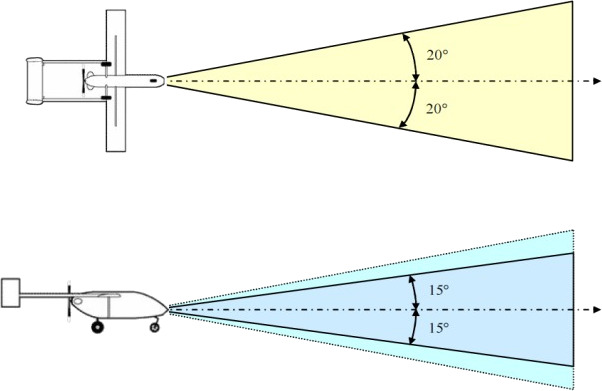
\includegraphics[width=.45\textwidth]{lidar_scan_ang} }
\subfigure[نحوه‌ی اسکن کردن محیط، در یک الگوی بیضوی با زوایایی مختلف، که امکان تشخیص موانع خطرناک مانند سیم‌های برق را می‌دهد.]{ 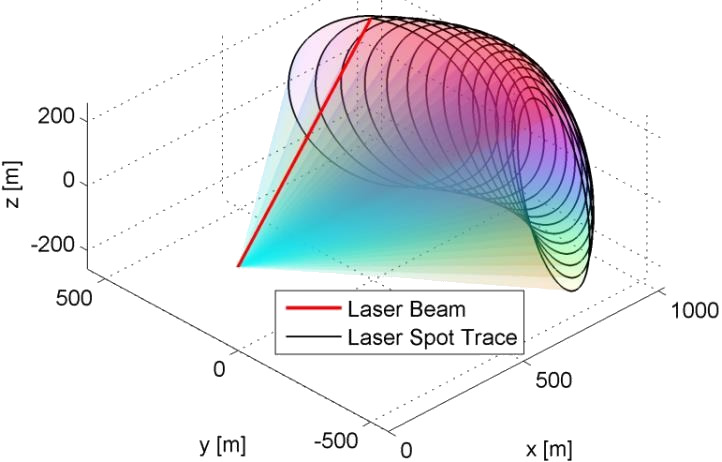
\includegraphics[width=.45\textwidth]{lidar_scan_pat} }
\caption{سیستم \مق{LOAM}}
\end{figure}

در پژوهشی دیگر در \سال{2016} به معرفی الگوریتم \جام تشک بادی محیطی\زیرنویس{\مق{Cushioned Extended-Periphery Avoidance}} پرداخته است که با استفاده از تعدادی حسگر لیزری که پیرامون ربات ۶پره مورد تحقیق بسته شده است، با در نظر گرفتن ۳ محور \جام، پرواز نرم و رسیدن به هدف، اقدام به \جام کرده است\مرجع{jackson2016cushioned}. این الگوریتم که به نوعی می‌توان جز تعمیم‌های الگوریتم \مق{PF} دانست که با همان ایدئولوژی‌ای که موانع نیروی پتانسیلی دافعه و هدف نیرو پتانسیل جازبه بروی ربات اعمال می‌کند، ارائه شده است. ایده‌ای جالبی که در این پژوهش سعی شده به آن بپردازد این است که هر مانعی در کنار اینکه دور یا نزدیک بدون آن می‌توان در شدت نیروی دافعه‌ای که به ربات اعمال می‌کند متغیر است، میزان نزدیکی به ربات در برآیند جهت نیروی دافعه‌ای آن مانع نیز تاثیرگذار است(شکل \ref{fig:cushion_forces}). همانطور که در شکل \ref{fig:cushion_sim} که نتیجه‌ی شبیه‌سازی این الگوریتم آمده است می‌بینیم پهپاد با نظر گرفتن میزان و جهت نیروی اعمال شده از طرف مانع به صورت دندانه‌ای\زیرنویس{Zikzak} به سمت هدف حرکت می‌کند، رفتاری که برای این گونه از محیط‌ها کاملا طبیعی می‌باشد.\بند

\begin{figure}
\centering
\subfigure[در ایده‌ی تشک بادی محیطی، برآیند نیروهای دافعه وارده به ربات از سمت یک مانع، وابسته به میزان نزدیکی ربات به آن مانع می‌باشد.]{ 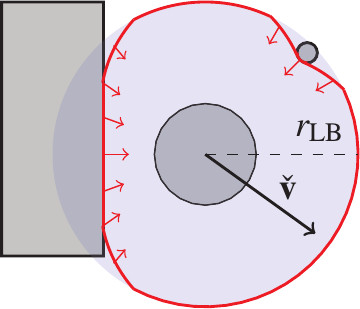
\includegraphics[width=.2\textwidth]{cushion_forces}\label{fig:cushion_forces} }
\subfigure[شبیه‌سازی انجام شده الگوریتم تشک بادی محیطی بروی یک محیط با موانع متعدد و نسبتا پیچیده]{ 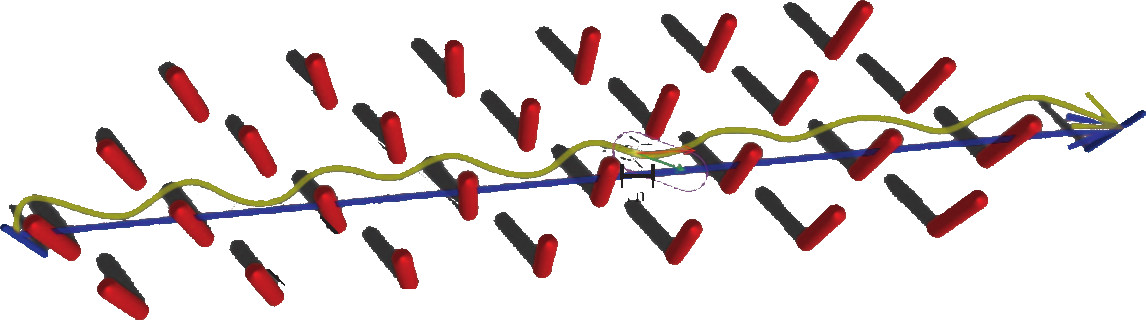
\includegraphics[width=.75\textwidth]{cushion_sim}\label{fig:cushion_sim} }
\caption{الگوریتم \جام تشک بادی محیطی}
\end{figure}
